\chapter{Evaluation}
\label{chapter:evaluation}

Before we evaluate the system, we will make a few notes that apply to the evaluation of the system as a whole.

\section{Notes}

All the tests and benchmarks were performed on a single machine.
The machine has 16GB of RAM, an M1 Apple Silicon processor 3200 MHz, and a 512GB SSD.
Due to these specs, the benchmarks are run with files between 1MB and 100MB.
We ran benchmarks with files up to 1GB and the results were consistent with the results from the smaller files,
i.e., the algorithms exhibit the same behavior, but rerunning the benchmarks takes a lot of time.

The system is written in Rust, which means no garbage collection or runtime overhead,
which we can see from running 1000 instances in \autoref{fig:1000-instances}.
Because the system consumes almost no resources when idle,
we can run many instances on a single machine.
We will not account for the overhead of the system being idle in the benchmarks.

\begin{figure}
    \centering
    \includegraphics[width=350pt]{gfx/1000-instances.png}
    \captionof{figure}{Starting 1000 instances}
    \label{fig:1000-instances}
\end{figure}

\section{PoR}

In this section, we will evaluate how the PoR system performs in a real-world scenario.
We have discussed how PoR is used to ensure the integrity of the data stored on the nodes.
Now, we will evaluate how viable is it to use PoR in the system.
Does it adhere to the \autoref{section:requirements}?
And is it fast enough to be used in a real-world scenario?

\subsection{How many audits can we perform in parallel?}

The audit is a two-step process.
First, the Verifier sends the challenge to the Keeper and then the Keeper responds with the proof.

We expect the load on the Verifier to be negligible, while the load on the Keeper to be significant.
The Verifier should do as little work as possible,
because we want to perform as many audits as possible in parallel.
This way we can ensure that audits are performed often enough to ensure the integrity of the data.
The load on the Keeper is expected to be high,
because the Keeper needs to read the file from disk and execute the PoR algorithm.
Ideally that algorithm will be linear in time complexity in the size of the file.

The Verifier performs 2 operations --- sending the challenge and verifying the proof.
We benchmarked these operations and the results are shown in \autoref{fig:por-verifier-create-challenge}
and \autoref{fig:por-verifier-audit-challenge}.

The results show that generating the challenge and auditing are both very fast operations ---
for a 100MB file, the Verifier can generate the challenge in 0.027ms and
audit the proof in 0.137ms.

We can observe something interesting the in the results ---
the graph looks almost logarithmic, instead of linear.
This is due to cache locality since both the operations are executing code on sequential memory addresses.
Both the challenge and the response are essentially a vector of numbers,
which is a very cache-friendly data structure.

\begin{figure}
  \myfloatalign
  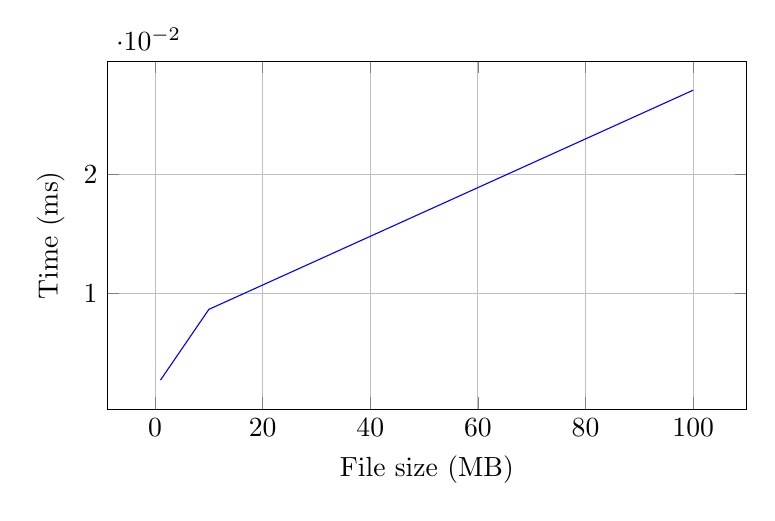
\begin{tikzpicture}
    \begin{axis}[
      xlabel={File size (MB)},
      ylabel={Time (ms)},
      grid=major,
      width=0.8\textwidth,
      height=6cm,
    ]
    \addplot[mark=., blue] coordinates {
      (1, 0.002736)
      (10, 0.008674)
      (100, 0.027069)
    };
    \end{axis}
  \end{tikzpicture}
  \caption[]{Time required for the Verifier to create the challenge for PoR.}
  \label{fig:por-verifier-create-challenge}
\end{figure}

\begin{figure}
  \myfloatalign
  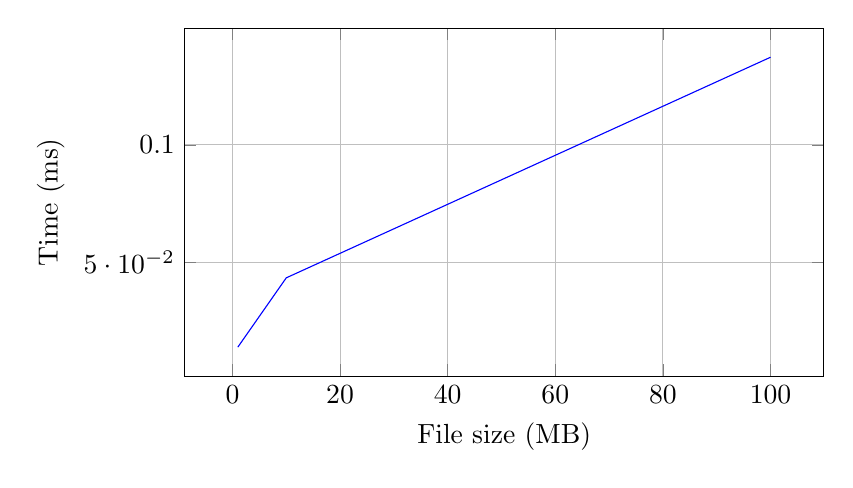
\begin{tikzpicture}
    \begin{axis}[
      xlabel={File size (MB)},
      ylabel={Time (ms)},
      grid=major,
      width=0.8\textwidth,
      height=6cm,
    ]
    \addplot[mark=., blue] coordinates {
      (1, 0.013733)
      (10, 0.043281)
      (100, 0.137354)
    };
    \end{axis}
  \end{tikzpicture}
  \caption[]{Time required for the Verifier to audit the challenge response PoR.}
  \label{fig:por-verifier-audit-challenge}
\end{figure}

The Keeper performs 1 operation --- generating the proof.
This is done by reading the file from disk and running the PoR algorithm on it.
The PoR algorithm is expected to be linear in time complexity in the size of the file.
We benchmarked this operation and the results are shown in \autoref{fig:por-keeper-challenge-generate}.

The operation gets slower as the file size increases.
In theory the time complexity should be linear, but it is superlinear in practice.
This is most likely caused by the unoptimized matrix multiplication algorithm that we are using to
implement PoR.

\begin{figure}
  \myfloatalign
  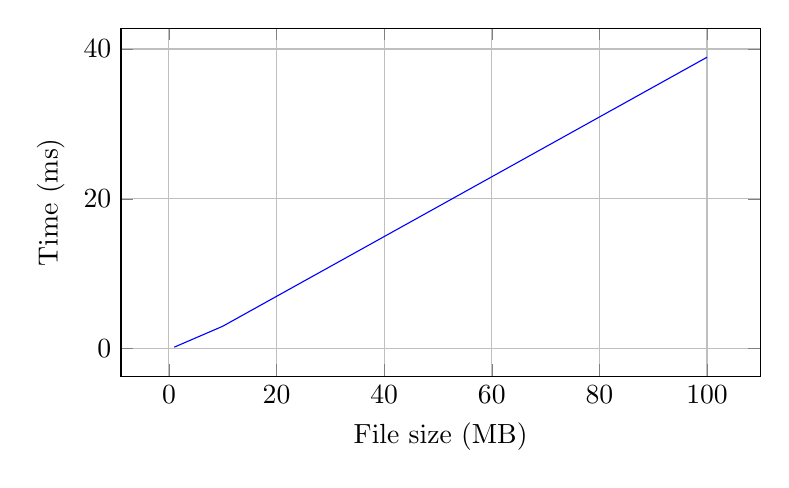
\begin{tikzpicture}
    \begin{axis}[
      xlabel={File size (MB)},
      ylabel={Time (ms)},
      grid=major,
      width=0.8\textwidth,
      height=6cm,
    ]
    \addplot[mark=., blue] coordinates {
      (1, 0.21614)
      (10, 3.002728)
      (100, 38.900041)
    };
    \end{axis}
  \end{tikzpicture}
  \caption[]{Time required to create the challenge response (proof) for PoR on the Keeper side, without reading the file from disk.}
  \label{fig:por-keeper-challenge-generate}
\end{figure}

\subsection{Is PoR the limiting factor in the system?}

In the previous section we saw that the Verifier can generate the challenge and audit the proof very quickly.
Since the speed of reading from an SSD is on average 7000 MB/s, the PoR protocol in the Verifier
will not affect the system's performance.
It is more likely, that the network connection between the Verifier and the Ledger will be the limiting factor,
but we will not evaluate network speeds as they are out of the scope of this thesis.

The Keeper can generate the proof at a rate of 38ms for a 100 MB.
This is faster than the access speed of an HDD, which is around 500 MB/s or 200ms for a 100 MB.
However, it is slower than the access speed of an SSD, which is around 7000 MB/s or 14ms for a 100 MB.
Whether the PoR protocol is the limiting factor or not depends on what kind of storage the Keeper is using.

In conclusion, the Verifier can send challenges in parallel, but the Keeper nodes will still be
the limiting factor in the system.

\section{TODO}
\wtf{WIP}

The next 3 questions:

    Is a reputation system based on a ledger a viable measure against malicious nodes?
    How does the validation system affect the performance of the network?
    Does the validation system affect the other features of the system (performance, security, etc.)?

\section{TODO}
\wtf{this section needs to be rewritten}

We need to evaluate the proper penalties and rewards for the nodes.
A good balance is needed between rewards and penalties to ensure that a node is
going to perform enough work for the system before being able to harm it.
Part of this evaluation will be:
\begin{enumerate}
    \item How much reputation points a node stakes when it stores a file?
    \item How much reputation points a node loses when it fails an audit?
    \item How much reputation points a node gains when it performs an audit?
    \item How much reputation points a node loses when it's discovered to not be performing audits?
    \item What is the starting reputation for new nodes?
    \item How do nodes increase their reputation at the very beginning?
    \item Does having high reputation give the node any benefits?
\end{enumerate}

Nodes with very high reputation could easily become malicious as they can absorb the penalties.
We need to solve this problem by either having a maximum reputation or by having the penalties be
percentage-based.

We need to answer the question of how often audits should be performed and how often nodes should
check the audit results of others.
The overhead of performing audits should be as low as possible, but the audits should be performed often enough
to ensure the integrity of the data.

Finding the balance between audits and the overhead of the audits, and the penalties and rewards for the nodes
is crucial for the success of the system.
We will evaluate the system by running it with different parameters and observing the behavior of the nodes.
We will discuss the details and the results of the evaluation in \ref{chapter:evaluation}.
